\chapter{Introduction}
\label{chap:introduction}
The most well-known and widely used asymmetric ('public-key') cryptographic scheme, published by the trio \name{Rivest}-\name{Shamir}-\name{Adleman} in 1977 and known as \glstext{rsa}, is based on the hardness assumption of the integer factorisation problem, factorising a large 2-composite number into its two prime factors $p$ and $q$ is believed to be hard \parencite{1983-rsa}.
As of today, this factorisation problem has not been proven to be in the \gls{np} complexity class, yet it is suspected that it might indeed be \gls{np}-complete (i.e. \hyperref[def:np-hard]{NP-hard} while still being in \gls{np}) when modelled using a traditional Turing machine.
Since the advent of quantum computation, this situation changed as a whole with Peter \name{Shor}'s algorithm \parencite{1997-shors-algorithm}, threatening the security of many cryptosystems, for instance \gls{rsa} which is still widely used today despite its known problems.

As it stands, lattice-based cryptography presents a solution to a politically and socially problematic situation in which few parties world-wide, with access to a sufficiently powerful quantum computer, may be able to decrypt most of today's digital communication.
\hyperref[subsec:lattice-crypto]{Lattice Cryptography} is based on other mathematical problems, shown to be sufficiently hard on quantum computers and traditional ones alike, most notably \hyperref[def:lwe-search-problem]{LWE} \parencite{2005-lwe-original} which this thesis will discuss in detail.

Many new cryptosystems have been developed on top of LWE, two of which this following thesis will focus on specifically: \hyperref[def:bfv-scheme]{BFV} and \hyperref[def:ckks-scheme]{CKKS};
whose security is still unaffected by efficient quantum algorithms.
Yet, it is not only their security prospect that makes these encryption schemes attractive, but first and foremost their defining \hyperref[def:ring-homomorphism]{homomorphic} property which allows for computations on the encrypted data.
A \glslink{fhe}{\textit{fully} homomorphic encryption} scheme was first introduced by Craig \name{Gentry} in 2009, using a bootstrapping approach \parencite{2009-gentry-fhe-original}.
The \textit{levelled} homomorphic \gls{bgv} encryption scheme is implemented in Microsoft SEAL and allows for integer arithmetic, up to a few multiplication 'levels' deep \parencite{2012-bgv-original}.
The \gls{bfv} scheme \parencite{2012-fv-original,2012-brakerski} is very similar to it and described in a bit more detail in \cref{sec:bfv}.
And finally, building upon concepts introduced in the former, the \gls{ckks} scheme \parencite{2017-ckks-original} allows for approximative floating-point arithmetic that finally facilitates machine-learning applications.

Machine Learning allows a computer to 'learn' from specifically structured data using linear regression or similar methods, and to apply this 'knowledge' to new, unknown inputs.
In its simplest form, or even using a multi-layered neural network, this only requires two different operations on numbers (or even better, vectors): addition and multiplication.
Using one of the \gls{he} schemes mentioned above and described in \cref{chap:homomorphic-encryption}, both are given and \gls{ppml} applications are born!

The present thesis not only focusses on theoretical remarks but also includes a publicly available implementation of an \gls{he} classification server written in C++, based on the \glsdesc{he} scheme \textit{SEAL} developed by Microsoft Research \parencite{seal-4.0}, and a compact graphical user interface to interact with.
A screenshot of the main functionality is displayed in \cref{fig:frontend}.

\begin{figure}[H]
  \centering
  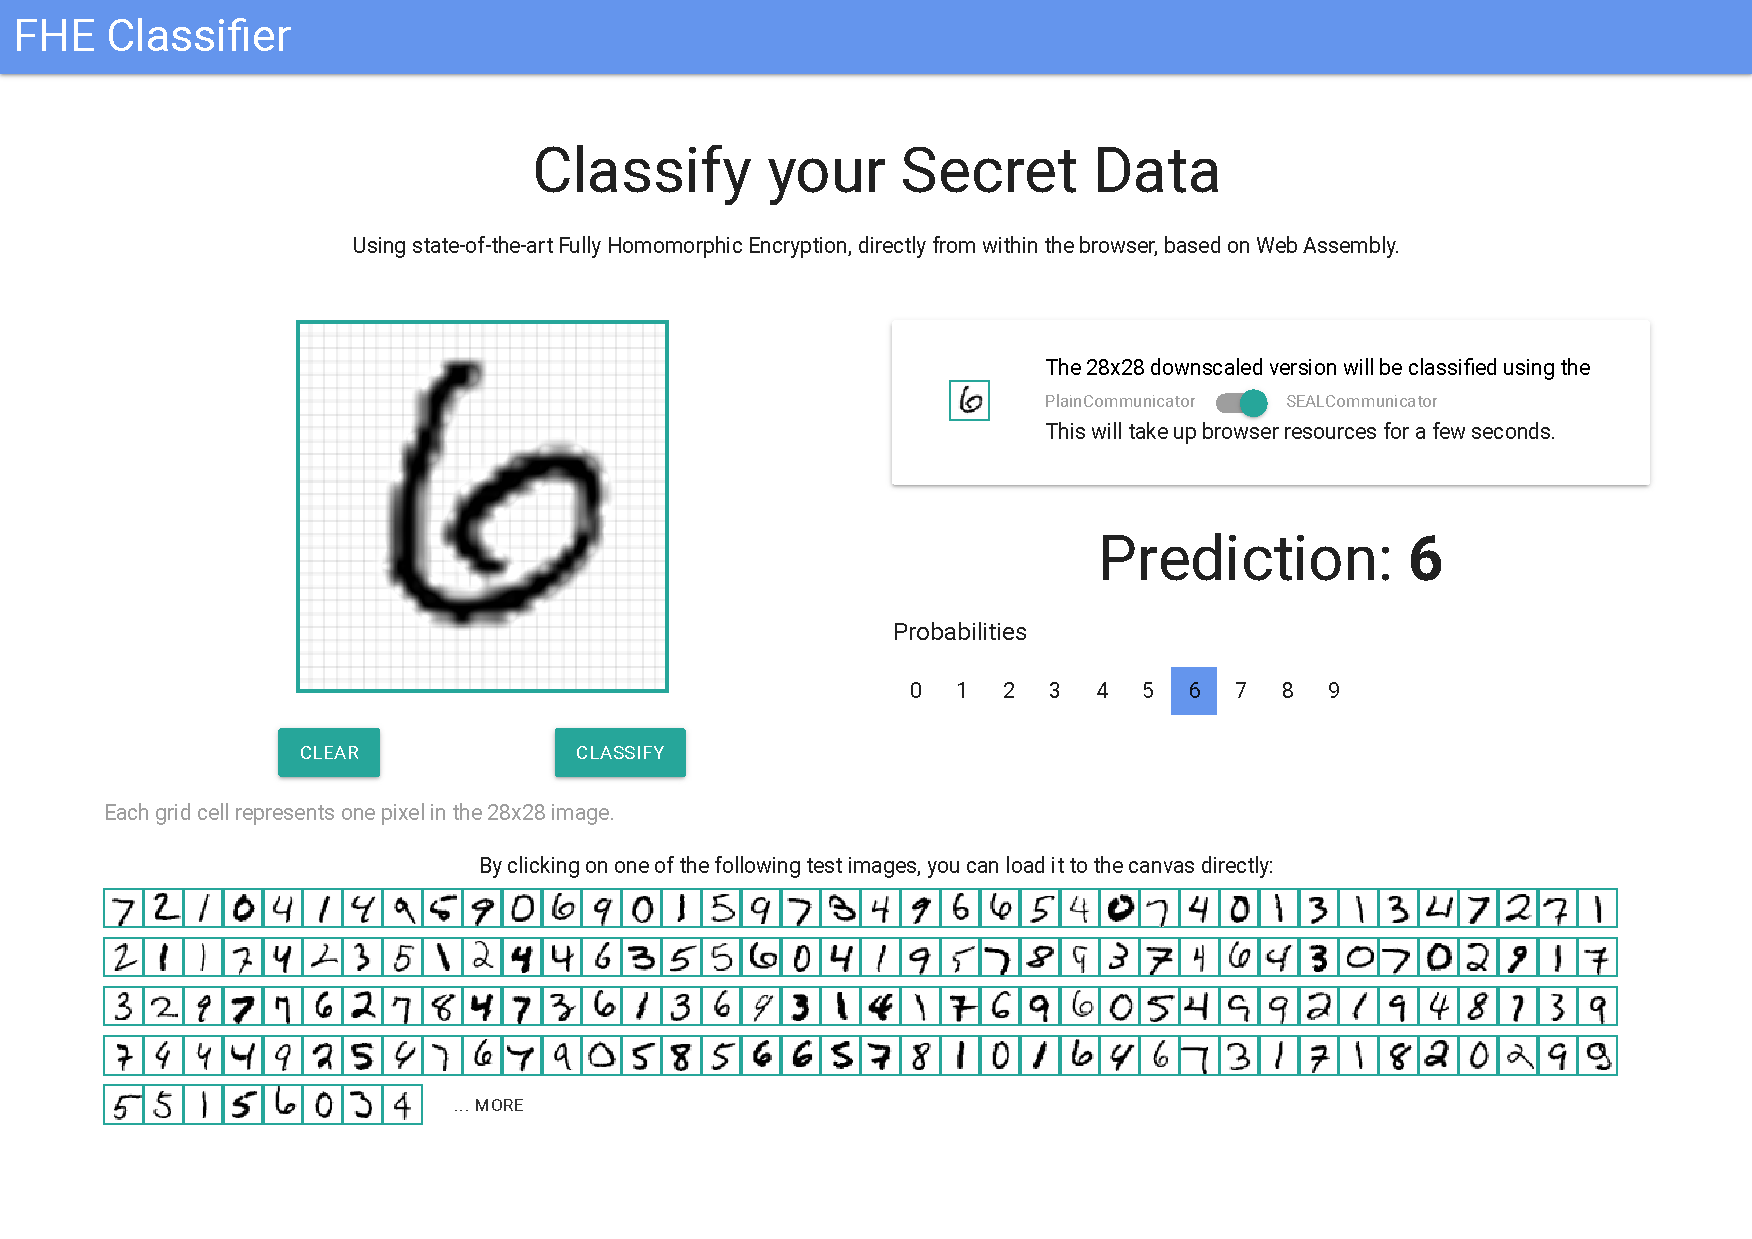
\includegraphics[width=\linewidth]{figures/frontend.pdf}
  \vspace{-1.2cm}
  \caption[User interface of the demonstrator]{The user interface of the demonstrator: users can draw a digit by hand, select one of two communication means (plain or encrypted) and finally let the server handle the classification to obtain a prediction (including a visual of associated probabilities).}
  \label{fig:frontend}
\end{figure}

The following \cref{chap:background} and \cref{chap:homomorphic-encryption} aim to introduce most of the necessary theory to understand the \gls{he} schemes used in practice today, as well as the simple machine learning approaches involved in securely classifying images as a service.

\Cref{chap:implementation} then focusses on the concrete system at hand, how the classification of handwritten digits (using the \glstext{mnist} dataset) works in detail and what challenges arise when dealing with a system which acts not only on plain, but also encrypted data.
\Cref{chap:results} analyses the neural network performance in terms of its accuracy, digit-wise precision and recall, documents benchmarks of runtime, message size and accuracy and finally includes a visualisation of the ciphertext (containing all information about the original image).
